\clearpage
\section{Project Phases}

The team mainly worked in phases called sprints. In the beginning of the project there were a 2 week period spent on preliminary studies and on planning. The next phases were the sprints (1-4). The sprints were scheduled to last for 2 weeks each with focus on the implementation of the game. The last phase was the delivery and documentation phase, where no new features were to be implemented. The phase was, however, spent ensuring that all code produced was ready for delivery and finishing the report.

\subsection{Planning and Research}
In this phase the focus was on getting started with the project. Every project need roles, a plan and a description of what to deliver. First roles were delegated. After delegating roles the game concept was developed, and the a requirement specification was made. Subsequently it had to be decided what technology to use, which methodology to follow as well as making an overall project plan. 

	\begin{figure}[H]
		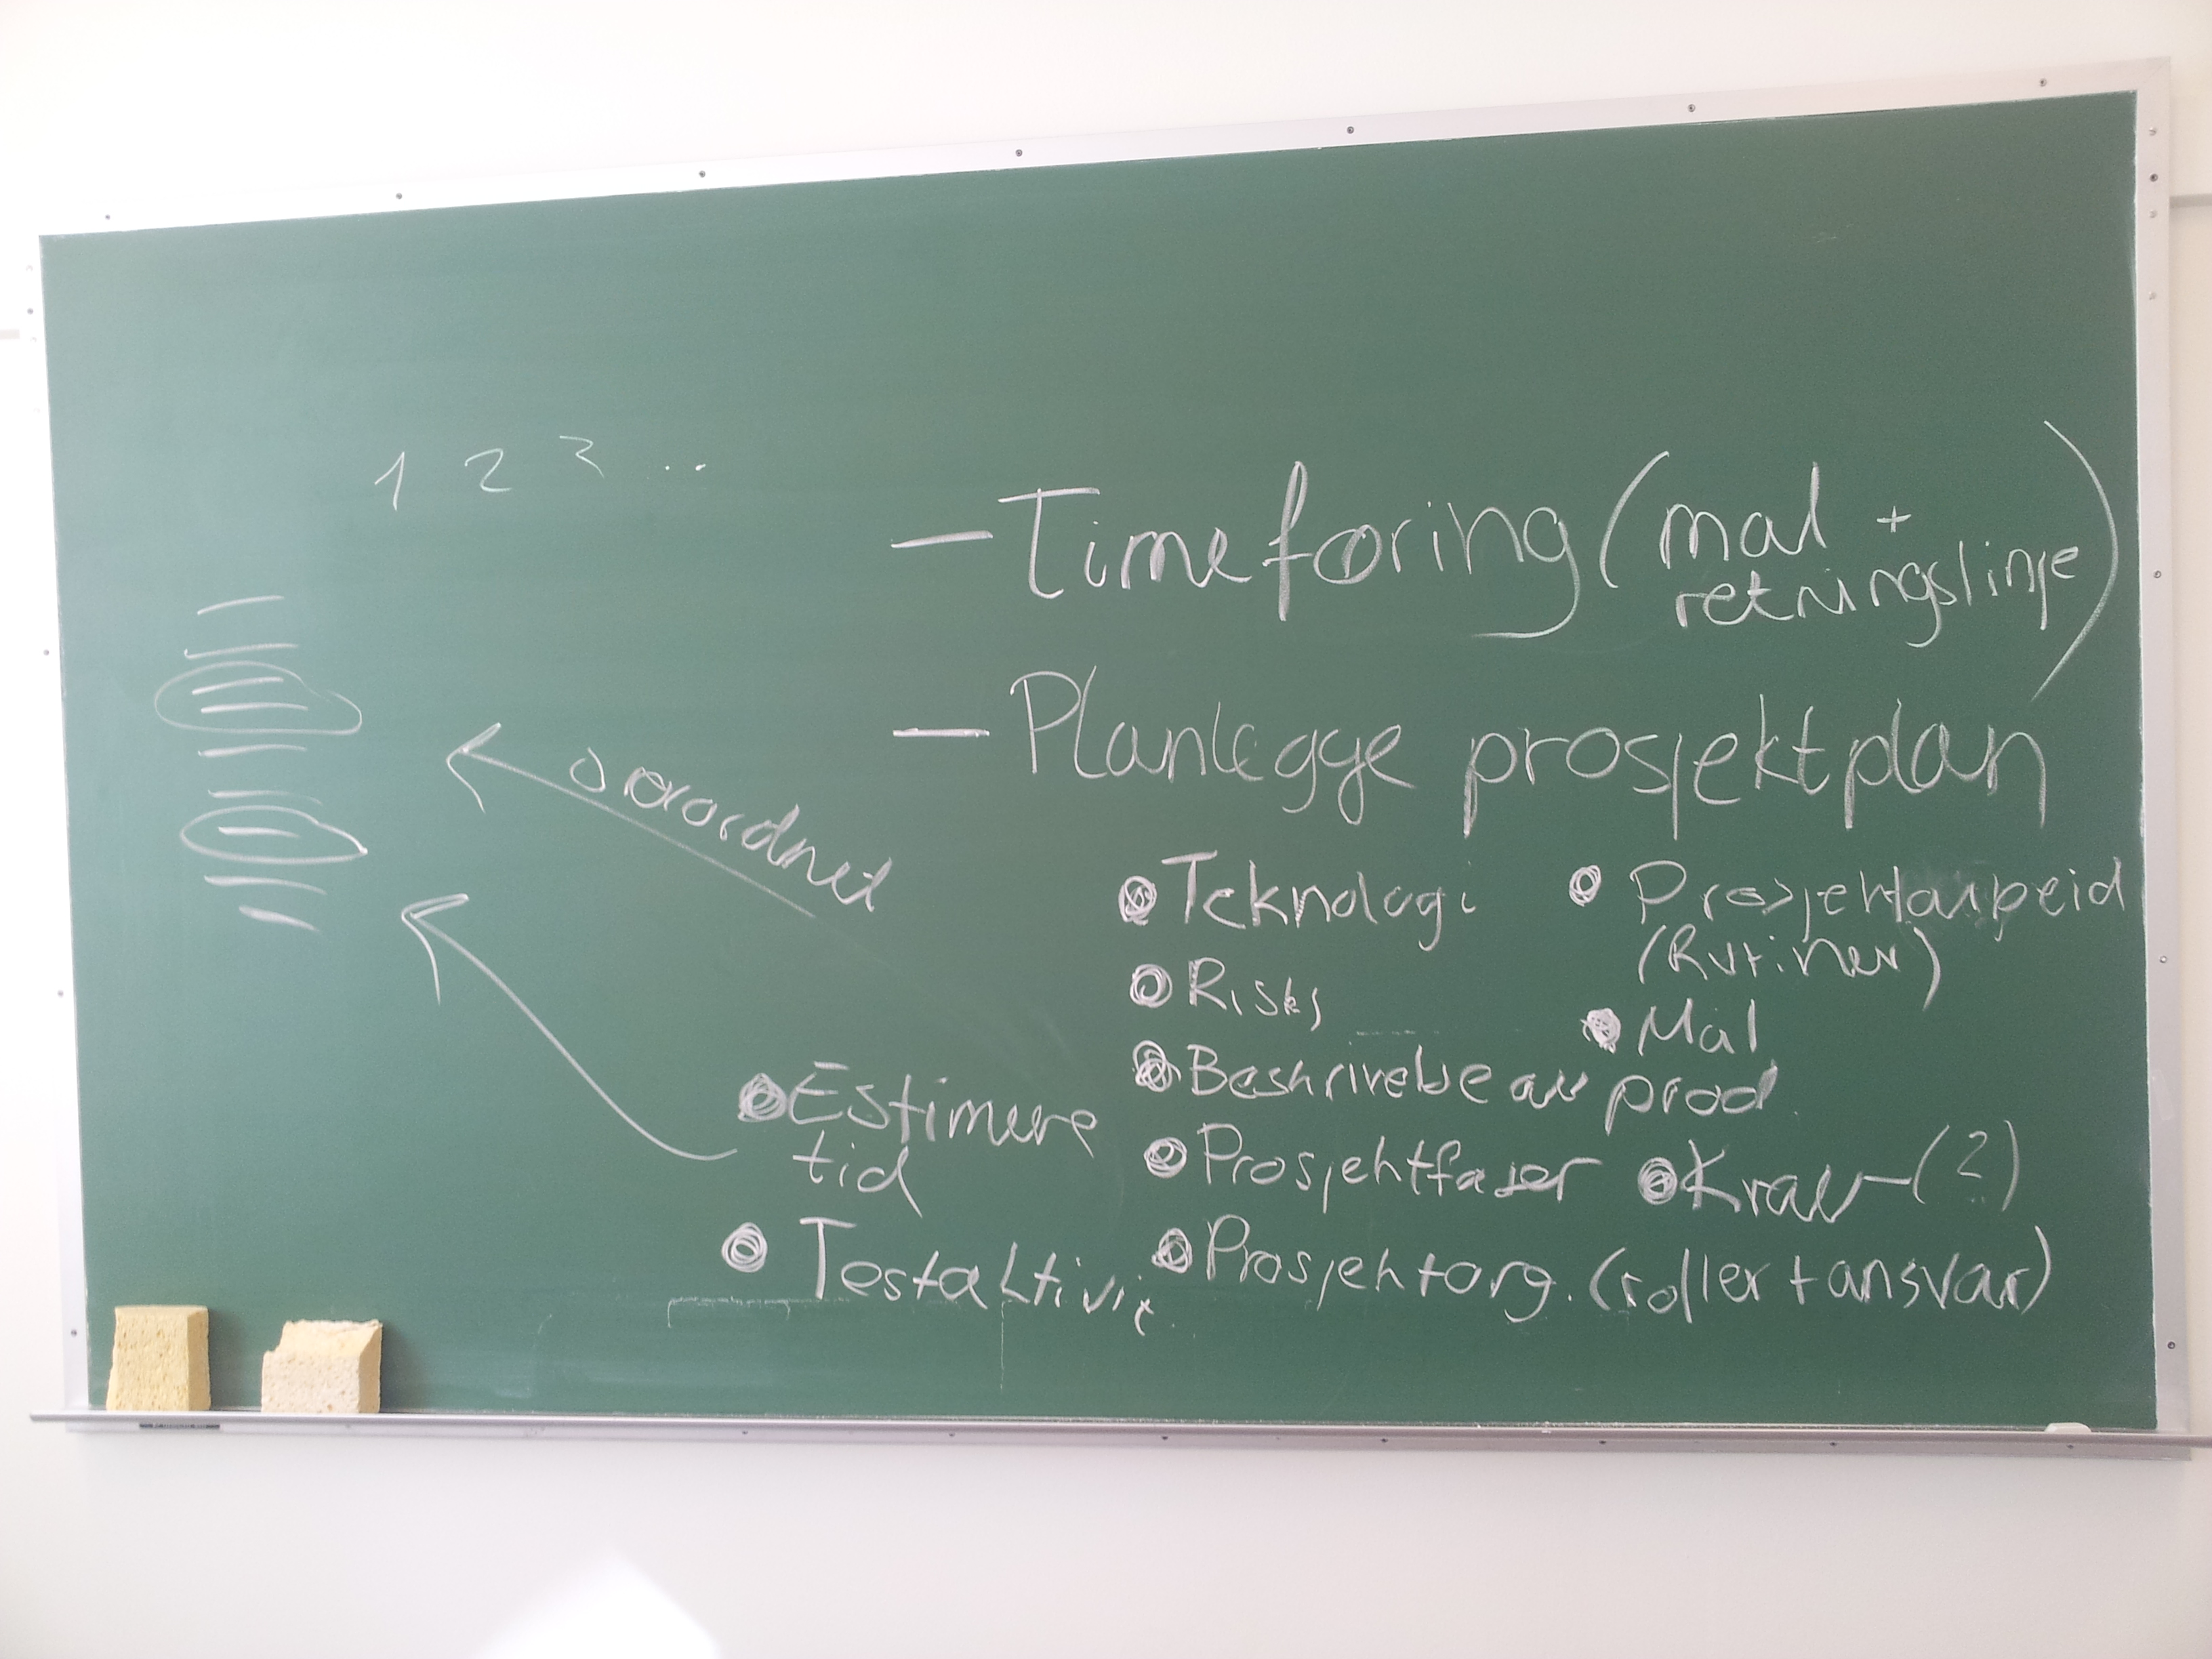
\includegraphics[scale=0.10]{pictures/projectPlanning.jpg}
		\caption{Group planning}
	\end{figure}

\subsection{Sprints}
This phase of the project was divided into 4 phases called sprints and which lasted 2 weeks each. In the sprints the focus was on what features to deliver at the end of the sprint as well as making progress with the report. The sprints and their activities and results are described as own chapters in the report.

\subsection{Documentation and Delivery}
This phase was the last week of the project. This is the time where no new features were implemented, but in which it was  made sure that the game was stable and playable. It was also important to finish the final documentation in this phase.
